% LaTeX schematics: Current Source
% Description: DC Current Source connected to Elmer Massive Coil
% Author: Jonathan Velasco, CSC - IT Center for Science
% Original date: September 2021
% email: jonathan.velasco@csc.fi
%------------------------------------------------------

%------------------------------------------------------
%         Document Settings
%------------------------------------------------------
\documentclass
[border=3mm]{standalone}

%------------------------------------------------------
%         Packages
%------------------------------------------------------

\usepackage[siunitx,cuteinductors,americanvoltages,americancurrents]{circuitikz}  

%------------------------------------------------------
%         Main
%------------------------------------------------------
\begin{document}     
        \begin{circuitikz}[PH/.append style={font=\scriptsize,inner ysep=2pt,inner xsep=5pt},
                           PV/.append style={PH,inner ysep=2pt,inner xsep=2pt}]
                
                \draw (0,0) % Begin Circuit
                
                % Ideal Sinusoidal Current Source
                to[I ,name=Is,-,l^=$\mathbf{I}$, v^={$$},thick] (0,4) (0,0)
                to[sinusoidal voltage source] (0,4) (0,0) 
                
                % Elmer FEM Component
                (0,4) node [PV,above left] {2} 
                to[generic, l^=$\mathbf{ElmerComponent}$,name=Ecomp,*-]  (4,4) 
                
                % Short Wires
                to[short,-] (4,0) 
                to[short,-] (2,0) node [ground]{} node [PV,above left] {1} (2,0) 
                to[short,*-] (0,0) ;
                
                % Component Values
                %\node[above, xshift=31pt, yshift=-14pt] at (Is.n) {1A};
                \node[below, xshift=2pt, yshift=-14pt] at (Ecomp.n) {Stranded Coil};
                

                \node[inner sep=0pt] (whitehead) at (8.5,2)
                    {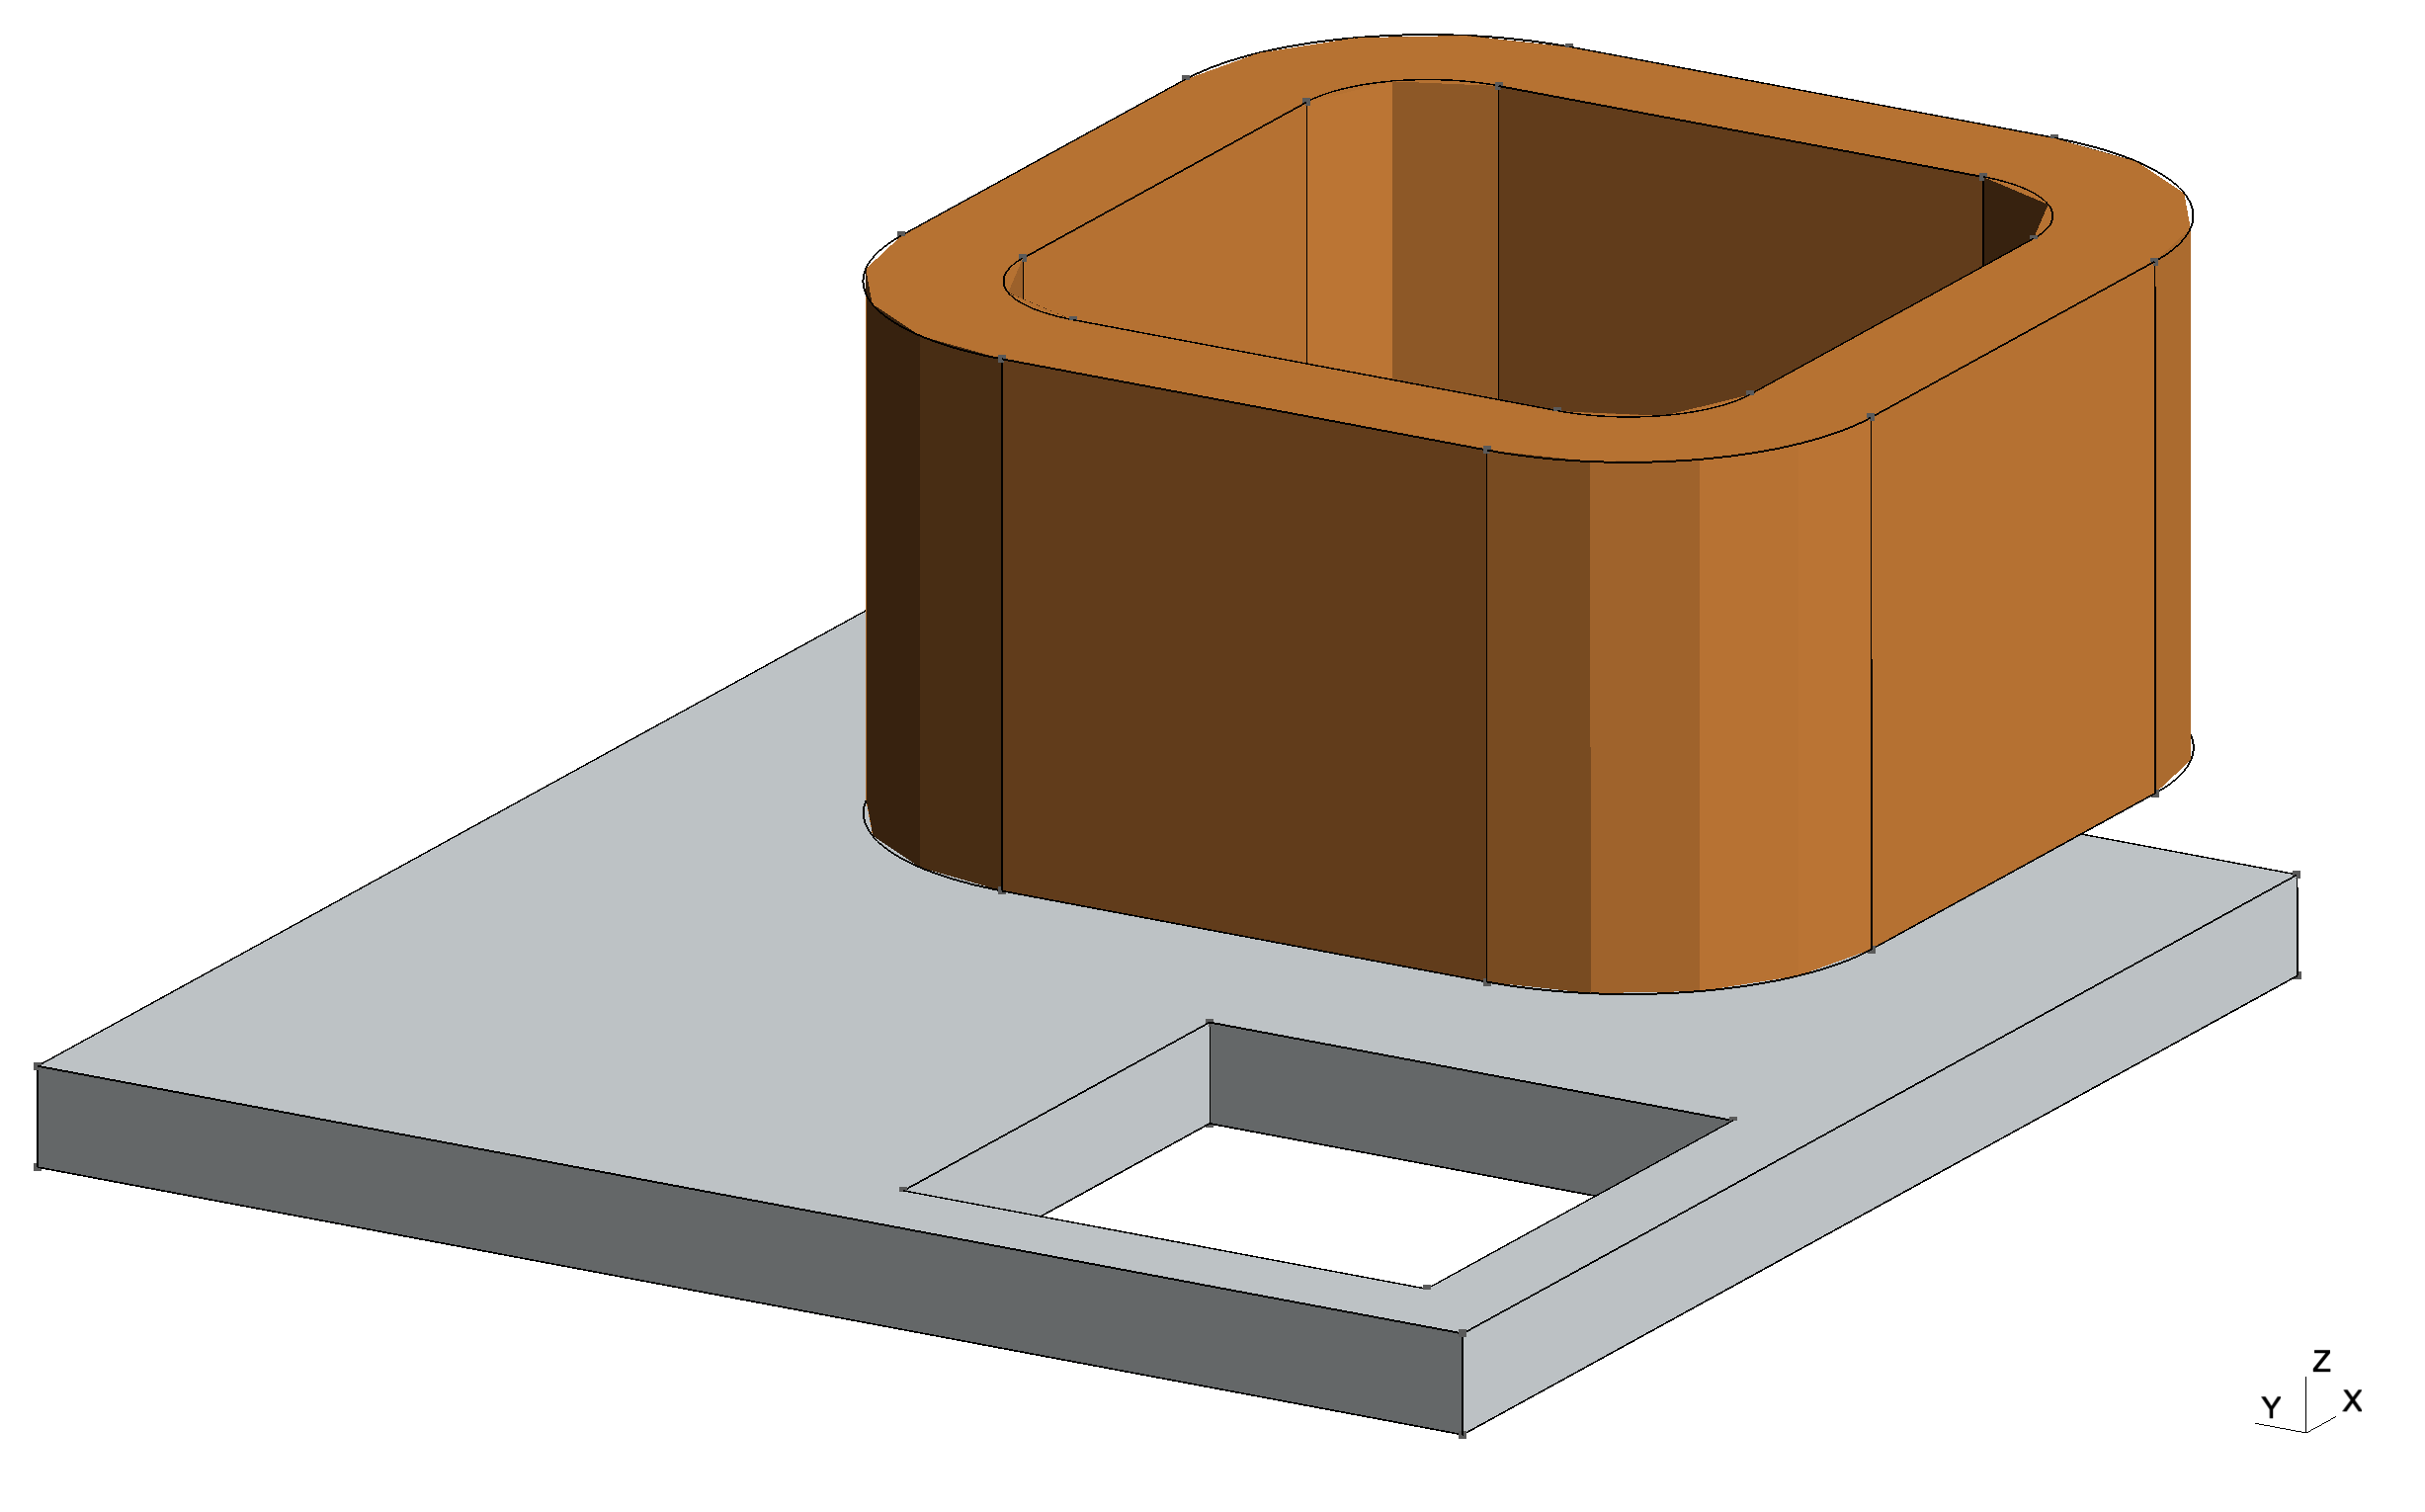
\includegraphics[width=.7\textwidth]{../tex-models/figures/TEAM7_geo.png}};
                    
                 % AC Current Source
                 \draw (5,2) % Begin Circuit
                to[I ,name=Is,-,l^=$\mathbf{I}$, v^={$$},thick] (5,4)
                 (5,2)
                 to[sinusoidal voltage source]  (5,4)
                 
                 to[short,-] (7.75,4)
                 (5,2)
                 to[short,-] (7.5,2);

        \end{circuitikz}
\end{document}

%------------------------------------------------------
%         EOF
%------------------------------------------------------